\documentclass[a4paper,12pt]{article}

\title{Chemistry 30 IB \\ Acids \& Bases}
\author{Jad Chehimi}

% document setup
\renewcommand{\familydefault}{\sfdefault}
\linespread{1.25}
\usepackage{setspace}
\usepackage{enumitem}
\setlist{nosep}

% tools
\usepackage{siunitx}
\usepackage[version=4]{mhchem}
\usepackage[hidelinks]{hyperref}
\usepackage{float}
%% images
\usepackage{graphicx}
\graphicspath{ {./images/} }

\usepackage[margin=1in]{geometry}

\begin{document}
\maketitle

% temp
\begin{center}
\Huge
Unfinished!
\normalsize
\end{center}
% temp

\tableofcontents

\pagebreak

\section{Theories}
The following two equations mean the same thing.

\ce{H+(aq)} and \ce{H3O+(aq)} are interchangable.

\subsection{Arrhenius}
\Large
$$\ce{HX(aq) -> H+(aq) + X-(aq)}$$
\normalsize
\begin{itemize}
    \item{doesn't specifically state water is present (aq)}
    \item{uses hydrogen ions, \ce{H+(aq)}}
    \item{cannot determine strong or weak}
\end{itemize}

\subsection{Br{\o}nsted-Lowry (aka. Modified Arrhenius)}
\Large
$$\ce{HX(aq) + H2O(l) -> H3O+(aq) + X-(aq)}$$
\normalsize
\begin{itemize}
    \item{specifically states water is present}
    \item{uses hydronium ions, \ce{H3O+(aq)}}
    \item{can determine strong or weak}
\end{itemize}

\section{General Equations}

\subsection{Ionization of Acids}
Forming ions from molecular compounds.

\subsubsection{Strong}
\Large
$$\ce{HX(aq) + H2O(l) ->[$>99.9\%$] H3O+(aq) + X-(aq)}$$
\normalsize
\begin{itemize}
    \item{ionize completely ($>99.9\%$ of the reaction completes)}
    \item{irreversible (\ce{->})}
    \item{high $K$ value ($K > 1$)}
\end{itemize}

\subsubsection{Weak}
\Large
$$\ce{HX(aq) + H2O(l) <=>[$<50\%$] H3O+(aq) + X-(aq)}$$
\normalsize
\begin{itemize}
    \item{do not ionize completely ($<50\%$ of the reaction completes)}
    \item{reversible (\ce{<=>})}
    \item{ionize at equilibrium}
    \item{low $K$ value ($K < 1$)}
\end{itemize}

\subsection{Dissociation of Bases}
Separation of existing ions in solution.

\subsubsection{Strong}
\Large
$$\ce{M(OH)_n + H2O(l) ->[$>99.9\%$] M^{n+}(aq) + nOH-(aq)}$$
\normalsize
\begin{itemize}
    \item{\ce{M} is a metal, \ce{M(OH)_n} is highly soluble}
    \item{dissociate quantitatively}
\end{itemize}

\subsubsection{Weak}
\Large
$$\ce{X(aq) + H2O(l) <=>[$<50\%$] HX+(aq) + OH-(aq)}$$
\normalsize
\begin{itemize}
    \item{dissociate at equilibrium}
\end{itemize}

\section{pH \& pOH}
\subsection{pH/pOH from Concentration}
\Large
$$\textrm{pH} = -\log{[\ce{H3O+}]}$$
$$\textrm{pOH} = -\log{[\ce{OH-}]}$$
\normalsize

\subsubsection{Shortcut}
The absolute value of the exponent of a concentration is the pH/pOH, for hydronium and hydroxide concentrations respectively.

e.g. $\SI{1.00e-4}{\mol\per\L}$ of \ce{H3O+} has a $\textrm{pH} = 4$

\subsection{Estimation}
This isn't required to know.

This only applies if the base is equal to 1.00. If the base is not 1.00, you can predict ranges that the pH/pOH could be. 

Of course, you can just calculate it, but this is a trick you can use to quickly figure out and compare pH/pOH from concentration.

\begin{itemize}
    \item{If $[\;\;] = 1$, then $\textrm{pH} = |exponent|$}
    \item{If $[\;\;] > 1$, then $\textrm{pH} < |exponent|$}
    \item{If $[\;\;] < 1$, then $\textrm{pH} > |exponent|$}
\end{itemize}


\subsection{Concentration from pH/pOH}
\Large
$$[\ce{H3O+}] = 10^{-\textrm{pH}}$$
$$[\ce{OH-}] = 10^{-\textrm{pOH}}$$
\normalsize

\subsection{Switching between pH and pOH}
\Large
$$\textrm{pH} + \textrm{pOH} = 14$$
\normalsize

\subsection{$K_w$}
The equilibrium constant of water can be used to solve for hydrogen ion concentration or hydronium ion concentration when you have the other.

$$K_w = [\ce{H3O+}][\ce{OH-}]$$

$$K_w = \SI{1.00e-14}{\mol\per\L}$$

$$\SI{1.00e-14}{\mol\per\L} = [\ce{H3O+}][\ce{OH-}]$$

\subsection{Significant Digits}
The significant digits of the concentration is the number of decimal pleaces of the pH/pOH.

For instance,
\begin{figure}[H]
    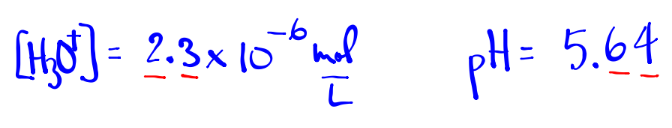
\includegraphics[width=\textwidth]{ph-sigdigs}
\end{figure}

\subsection{Square}
This may help you remember when to use what.
\begin{figure}[H]
    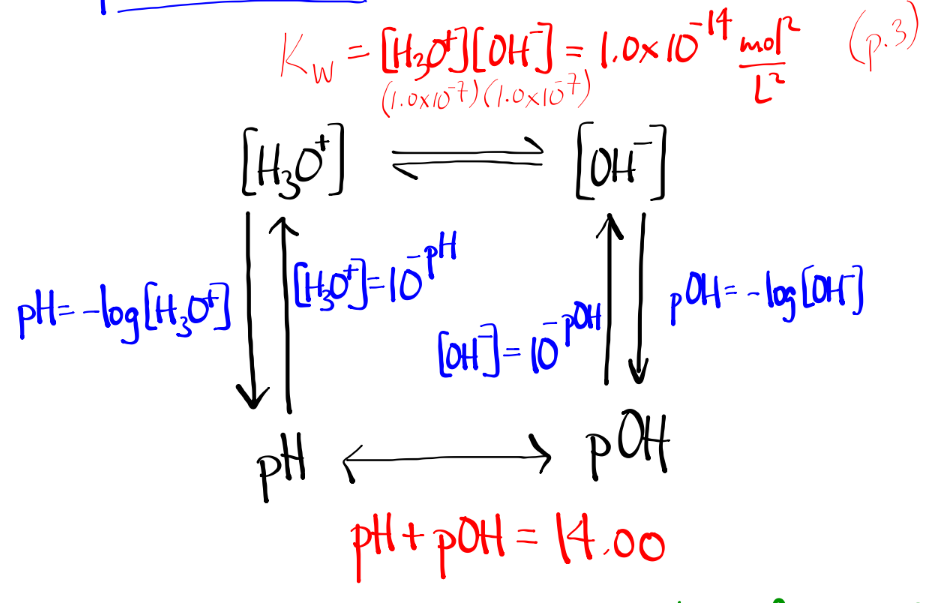
\includegraphics[width=\textwidth]{ph-square}
\end{figure}

\subsection{Example}
\begin{figure}[H]
    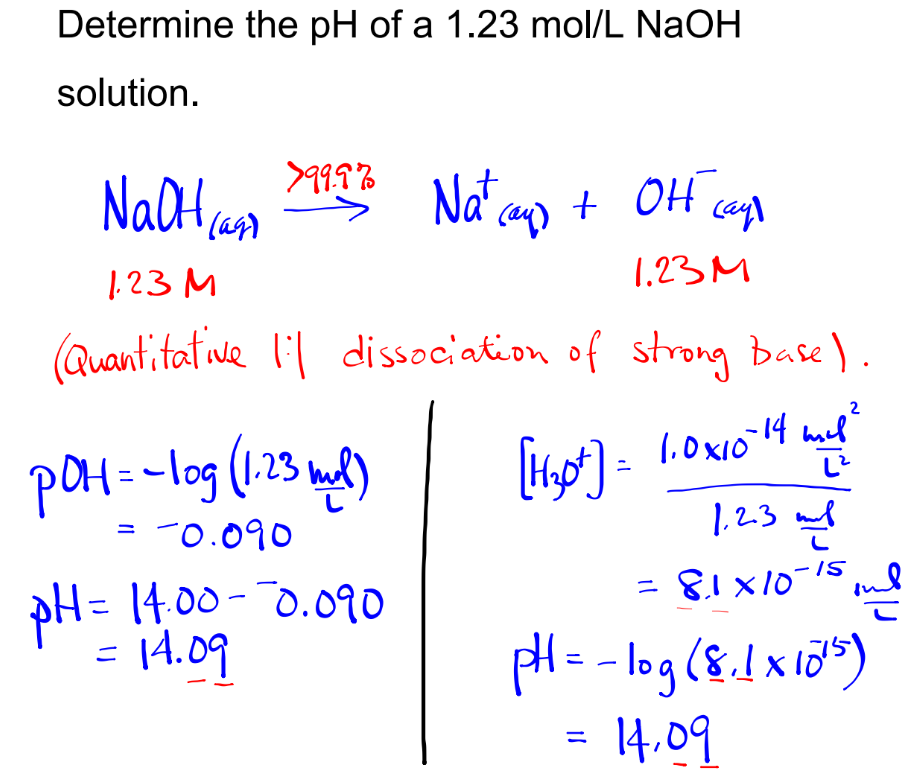
\includegraphics[width=\textwidth]{ph-example}
\end{figure}

\section{Acid/Base Reaction}
Also known as a neutralization reaction.

The complete or partial transfer of protons (\ce{H+}) from the strongest acid to the strongest base. The acids donate protons, the bases accept protons.

\normalsize
\begin{figure}[H]
    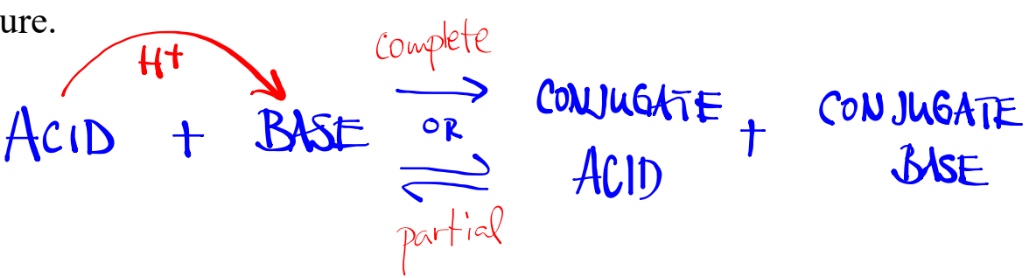
\includegraphics[width=\textwidth]{acidbase}
\end{figure}

\subsection{Net Reaction}
At this level, we typically only see the net reaction.

For your information, this is what leads to the net reaction.
\begin{figure}[H]
    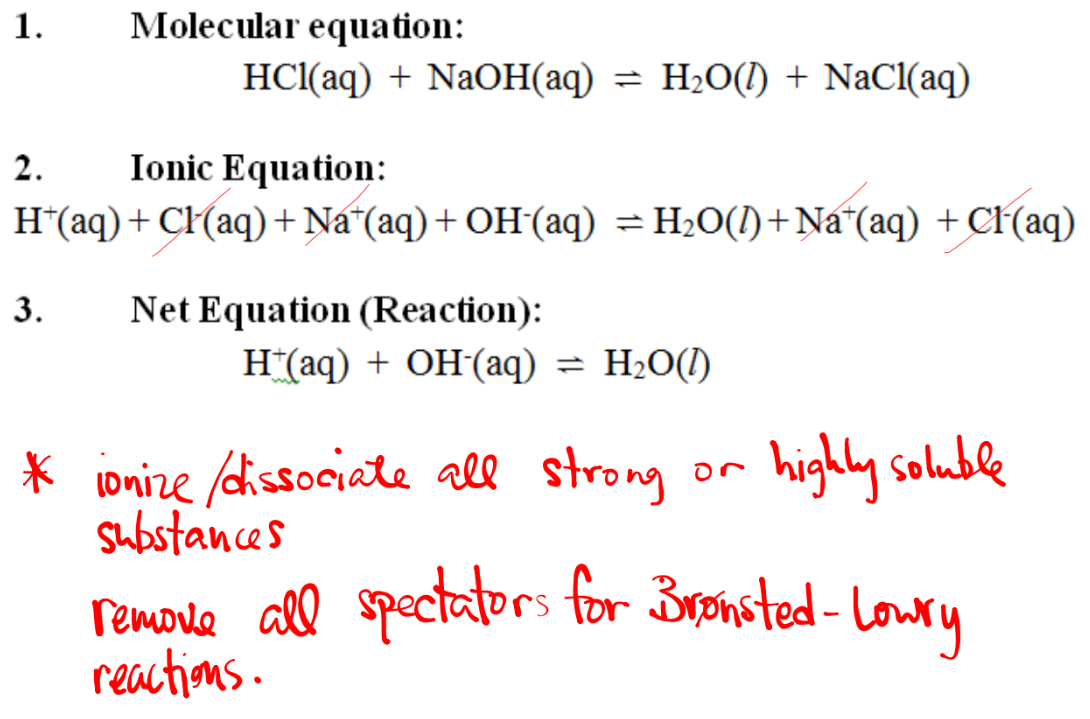
\includegraphics[width=\textwidth]{net}
\end{figure}

\pagebreak

\subsection{Conjugate}
\begin{itemize}
    \item{The conjugate base (CB) is what an acid becomes on the product side.}
    \item{The conjugate acid (CA) is what a base becomes on the product side.}
\end{itemize}

Conjugates differ from their original by one proton. (\ce{H+})

This is because, say a compound loses a proton from left to right, then it is an acid. Read that in reverse, right to left, and it gains a proton, making it a base.
\begin{figure}[H]
    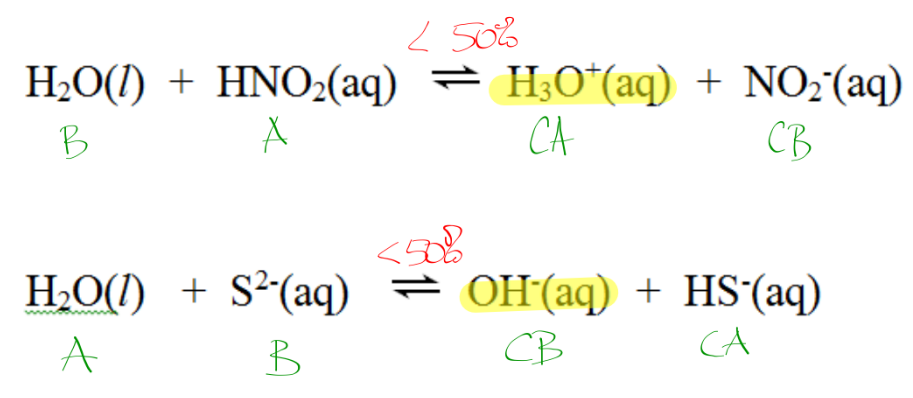
\includegraphics[width=\textwidth]{conjugate}
\end{figure}

A conjugate pair would be either,
\begin{itemize}
    \item{an acid and its conjugate base}
    \item{a base and its conjugate acid}
\end{itemize}

\subsection{Polyprotic Acids}
Acids that can donate a proton more than once.

They do it one at a time, yielding a different $K_a$ value every time.

\begin{itemize}
    \item{$\ce{H2CO3(aq) + H2O(l) <=> H3O+(aq) + HCO3-(aq)} \;\;\;\;\;\; K_a = \num{4.4e-7}$}
    \item{$\ce{HCO3-(aq) + H2O(l) <=> H3O+(aq) + CO3^{2-}(aq)} \,\;\;\;\;\;\; K_a = \num{4.7e-11}$}
\end{itemize}

For calculating the pH of a polyprotic acid, the $K_a$ of the first ionization should be used for calculations.

The conjugate base of polyprotic acids are amphiprotic.

\subsection{Amphiprotic}
Sometimes called amphoteric. Water is amphiprotic.

Substances that are both a base and an acid. Whether they behave as an acid or a base depends on the other substance in the acid/base reaction. 

It will do the opposite of the other substance, so if it were an acid, the amphiprotic will behave as a base, and vice versa.

Amphiprotics also often are a negative ion with hydrogen---\ce{HX-}---such as \ce{HSO4-(aq)}.

If both substances in an acid/base reaction can behave as an acid, the stronger acid will behave as an acid, the other as a base.

\subsection{Favourability}
\subsubsection{Hydronium or Hydroxide Present}
If \ce{H3O+} or \ce{OH-} are present, the reaction will favour the side they are not on.

If either one of these two ions are,
\begin{itemize}
    \item{a reactant, then products are favored. \ce{->[$>99.9\%$]}}
    \item{a product, then reactants are favored. \ce{<=>[$<50\%$]}}
\end{itemize}

\subsubsection{No Hydronium/Hydroxide}
On page 8-9 in your data booklet,
\begin{itemize}
    \item{if the acid is above the base, then products are favored. \ce{->[$>99.9\%$]}}
    \item{if the base is above the acid, then reactants are favored. \ce{<=>[$<50\%$]}}
\end{itemize}

The higher on the table, the stronger the acid. If the acid is stronger, it'll more likely donate protons, increasing the concentration of the opposing side of the reaction.

\section{(AB) Relative Strength}
The following is, oddly enough, non-IB.

\begin{itemize}
    \item{$K_a$ = acid equilibrium constant \\ how much \ce{H3O+(aq)} is produced when an acid interacts with water}
    \item{$K_b$ = base equilibrium constant \\ how much \ce{OH-(aq)} is produced when an base interacts with water}
\end{itemize}

Equilibrium constants are calculated the same as usual. Product of concentrations of products divided by product of concentrations of reactants, not including liquid water.

\subsection{$K_a$ of Common Substances}
The equilibrium constant of many common acids is provided on page 8-9 of the Alberta data booklet, on the right-most column.

But what if you want $K_b$?

\subsection{Converting between acid/base equilibrium constants}
\Large
$$K_w = K_a \times K_b$$
\normalsize

This means you can calculate $K_b$ as long as you have $K_a$, since $K_w$ is a known constant.

The $K_a$ of a base on the table is actually the conjugate acid. Doesn't really change anything---they are on the same line, after all---but good to know.

\Large
$$K_b = \frac{\SI{1.0e-14}{\mol\per\L}}{K_a}$$
\normalsize

If the $K_b > K_a$, than the base is a stronger base than the conjugate is an acid. This doesn't always mean its a base---its just a stronger base.

\subsubsection{Example}
The target base is ammonia, \ce{NH3}. The conjugate acid of ammonia, ammonium \ce{NH4+}, has a $K_a$ listed on the table---\SI{5.6e-10}{\mol\per\L}.

Therefore,
$$K_b = \frac{\SI{1.0e-14}{\mol\per\L}}{\SI{5.6e-10}{\mol\per\L}}$$
$$K_b = \SI{1.7e-5}{\mol\per\L}$$
Ammonia \ce{NH3} is a stronger base than ammonium \ce{NH4+} is an acid.

\section{pH/pOH and Ion Concentration of Weak Acids/Bases}
\subsection{Strong}
Strong acids and bases ionize/dissociate completely, respectively. The concentrations of the acid/base is equal to the concentration of hydronium/hydroxide ions. They ionize/dissociate quantitatively.

\begin{center}
    $[\textrm{acid}] = [\ce{H3O+}]$ \hspace{1in} $[\textrm{base}] = [\ce{OH-}]$
\end{center}

\subsection{Weak}
If you want the full explanation of where these formulas are derived from, read the actual notes---page 38. The following are the shortcuts you truly only need.

\subsubsection{Known Ion Concentration}
The following should be used if you know the ion concentration or pH/pOH, since pH/pOH can be converted into ion concentration.

\begin{center}
\Large
$K_a = \frac{[\ce{H3O+}]^2}{[\textrm{acid}] - [\ce{H3O+]}}$
\hspace{0.5in}
$K_b = \frac{[\ce{OH-}]^2}{[\textrm{base}] - [\ce{OH-]}}$
\normalsize
\end{center}

\subsubsection{Unknown Ion Concentration}
If you are solving for ion concentration with the aforementioned formula, you will require the quadratic formula. To avoid this, the ion concentration in the denominator can be omitted, since it affects the calculation negligably.

\begin{center}
\Large
$K_a = \frac{[\ce{H3O+}]^2}{[\textrm{acid}]}$
\hspace{0.5in}
$K_b = \frac{[\ce{OH-}]^2}{[\textrm{base}]}$
\normalsize
\end{center}

Therefore, you can now find ion concentration of weak acids/bases.

\begin{center}
\Large
$[\ce{H3O+}] = \sqrt{K_a \cdot [\textrm{acid}]}$
\hspace{0.5in}
$[\ce{OH-}] = \sqrt{K_b \cdot [\textrm{base}]}$
\normalsize
\end{center}



\end{document}
